\chapter{Phân tích và thiết kế hệ thống}
\label{chap:thiet_ke}

Chương này trình bày yêu cầu, chức năng, kiến trúc, các luồng xử lý, các thành phần, mô hình dữ liệu và giao diện của hệ thống.

\section{Yêu cầu của hệ thống}
\label{sec:yeu-cau}

\subsection{Đối tượng sử dụng}

Hệ thống phục vụ ba nhóm đối tượng. \textbf{Người dùng cuối} mô tả món đồ bằng tiếng Việt hoặc tải một ảnh mẫu lên, rồi nhận danh sách sản phẩm gần nhất trong catalog qua giao diện web. \textbf{Developer} là các thành viên của nhóm; họ lập chỉ mục catalog, chạy đánh giá, kiểm định thống kê và tinh chỉnh mô hình (FR05 đến FR08). \textbf{Người gán nhãn} chấm điểm liên quan 0, 1 hoặc 2 cho từng cặp truy vấn--sản phẩm (FR09). Hệ thống không có tài khoản; dịch vụ chạy cục bộ, có thể bảo vệ bằng một khoá API dùng chung.

\subsection{Yêu cầu chức năng}

Bảng~\ref{tab:c3_fr} liệt kê chín yêu cầu chức năng; bốn yêu cầu đầu dành cho người dùng cuối, năm yêu cầu sau phục vụ việc xây dựng và so sánh các hệ tìm kiếm.

\begin{table}[!htbp]
\centering
\caption{Yêu cầu chức năng}
\label{tab:c3_fr}
\footnotesize
\renewcommand{\arraystretch}{1.0}
\begin{tabularx}{\textwidth}{@{}p{1.2cm} >{\raggedright\arraybackslash}X p{2.6cm}@{}}
\toprule
\textbf{Mã} & \textbf{Yêu cầu} & \textbf{Tác nhân} \\
\midrule
FR01 & Tìm sản phẩm bằng mô tả tiếng Việt dài từ 1 đến 512 ký tự; trả về $K$ kết quả ($K$ từ 1 đến 100), xếp hạng và kèm điểm tương đồng & Người dùng cuối \\
FR02 & Tìm sản phẩm bằng ảnh tải lên, tối đa 8 MiB; chỉ áp dụng khi cấu hình dùng bộ tìm kiếm vector, vì BM25 từ chối truy vấn chỉ có ảnh & Người dùng cuối \\
FR03 & Lọc kết quả theo một danh mục, cho cả tìm bằng chữ và tìm bằng ảnh & Người dùng cuối \\
FR04 & Hiển thị trạng thái hệ thống: tên bộ tìm kiếm, số sản phẩm đã lập chỉ mục, và trạng thái suy giảm khi kho vector không trả lời & Người dùng cuối \\
FR05 & Lập chỉ mục catalog bằng mô hình đã đăng ký: mã hoá ảnh sản phẩm và ghi vào kho theo từng lô; có tuỳ chọn xoá rồi tạo lại bộ sưu tập (collection, nhóm vector cùng chiều trong kho) & Developer \\
FR06 & Chạy một hệ tìm kiếm trên bộ truy vấn, lưu 20 kết quả đầu, tính Recall@1/5/10, MRR, nDCG@10 và ghi nhật ký thí nghiệm & Developer \\
FR07 & Kiểm định chênh lệch giữa hai hệ bằng bootstrap ghép cặp theo truy vấn (lấy mẫu lại các truy vấn); tính hệ số kappa giữa những người chấm & Developer \\
FR08 & Tinh chỉnh SigLIP~2 bằng LoRA hoặc DoRA; dùng GradCache (tích luỹ gradient theo từng khối nhỏ) để huấn luyện với kích thước lô lớn; lưu lại bản trọng số có Recall@5 cao nhất trên tập xác thực & Developer \\
FR09 & Gán nhãn mù 0/1/2 cho cặp truy vấn--sản phẩm, ghi riêng theo từng người chấm, cho phép hoàn tác điểm vừa chấm & Người gán nhãn \\
\bottomrule
\end{tabularx}
\end{table}

\subsection{Yêu cầu phi chức năng}

Bảng~\ref{tab:c3_nfr} nêu các yêu cầu phi chức năng cùng chỉ tiêu. NFR04 và NFR02 chi phối kiến trúc nhiều nhất. NFR04 buộc mọi hệ được đo trong cùng điều kiện, nếu không bảng xếp hạng không có giá trị so sánh; NFR02 buộc hệ thống chạy được trên máy cá nhân để người khác tái lập đồ án.

\begin{table}[!htbp]
\centering
\caption{Yêu cầu phi chức năng và chỉ tiêu}
\label{tab:c3_nfr}
\footnotesize
\renewcommand{\arraystretch}{1.0}
\begin{tabularx}{\textwidth}{@{}p{1.3cm} p{2.3cm} >{\raggedright\arraybackslash}X >{\raggedright\arraybackslash}X@{}}
\toprule
\textbf{Mã} & \textbf{Thuộc tính} & \textbf{Yêu cầu} & \textbf{Chỉ tiêu} \\
\midrule
NFR01 & Độ trễ & Một truy vấn chữ trả kết quả đủ nhanh để dùng tương tác & p95 của thời gian mã hoá và tìm dưới 200 ms trên máy phát triển, với kho trong bộ nhớ. Đề cương không nêu phân vị nên đồ án chọn p95 \\
NFR02 & Chạy nhẹ & Lõi, API web và bộ kiểm thử chạy được với các gói nhẹ, không cần GPU, Qdrant hay tải mô hình & Khởi động bằng cấu hình mặc định; bộ kiểm thử mặc định chạy không lỗi \\
NFR03 & Khả năng thay thế & Thêm một mô hình hoặc một kho vector mới không phải sửa lõi & Mọi bộ mã hoá và kho vector đi qua cùng một bộ tìm kiếm vector của lõi; thêm bộ chuyển đổi mới chỉ cần thêm một tệp và khai báo trong bộ đăng ký \\
NFR04 & So sánh được & Mọi hệ dùng chung cổng tìm kiếm, bộ truy vấn và định nghĩa chỉ số & Các hệ dùng chung một tệp truy vấn và một tệp nhãn \\
NFR05 & Tái lập & Cấu hình tập trung; mỗi lần chạy được ghi lại & Giá trị khởi tạo ngẫu nhiên cố định; mỗi lần đánh giá hoặc huấn luyện thêm một dòng vào nhật ký 16 cột \\
NFR06 & Bảo mật đầu vào & Khoá API tuỳ chọn; giới hạn kích thước đầu vào & Khi đặt khoá, khoá sai bị từ chối (401); ảnh quá 8 MiB bị từ chối (413), ảnh rỗng (422) \\
NFR07 & Chịu lỗi kho vector & Mất kết nối kho không làm sập API web & Trạng thái hệ thống báo suy giảm; tìm kiếm trả 503 với thông báo cố định, không lộ địa chỉ kho \\
NFR08 & Quy mô catalog & Phục vụ catalog có quy mô như đề cương nêu & 20.000 đến 50.000 sản phẩm \\
\bottomrule
\end{tabularx}
\end{table}

Mức đạt của từng yêu cầu được đối chiếu ở Mục~\ref{sec:ke-hoach-kiem-thu} của Chương~\ref{chap:danh_gia}. Hai yêu cầu chưa đạt là NFR08, do catalog thực tế chỉ có 6.963 ảnh, và NFR01 với hệ DoRA; số đo của NFR01 nằm ở Chương~\ref{chap:danh_gia}.

\section{Chức năng và kịch bản sử dụng}
\label{sec:chuc-nang}

Hình~\ref{fig:c3_chucnang} nối chín chức năng với ba tác nhân. Người dùng cuối dùng FR01 đến FR04 qua giao diện web; Developer và người gán nhãn dùng các công cụ dòng lệnh và một máy chủ gán nhãn nhỏ chạy cục bộ. Trong chín chức năng, lọc theo danh mục (FR03) và kiểm định thống kê (FR07) là tuỳ chọn; bảy chức năng còn lại cần có để hệ thống tìm kiếm và đánh giá hoạt động. Bảng~\ref{tab:c3_uc01} và Bảng~\ref{tab:c3_uc02} mô tả hai kịch bản của người dùng cuối; luồng lập chỉ mục của Developer nằm ở Mục~\ref{sec:luong-xu-ly}.

\begin{figure}[!htbp]
\centering
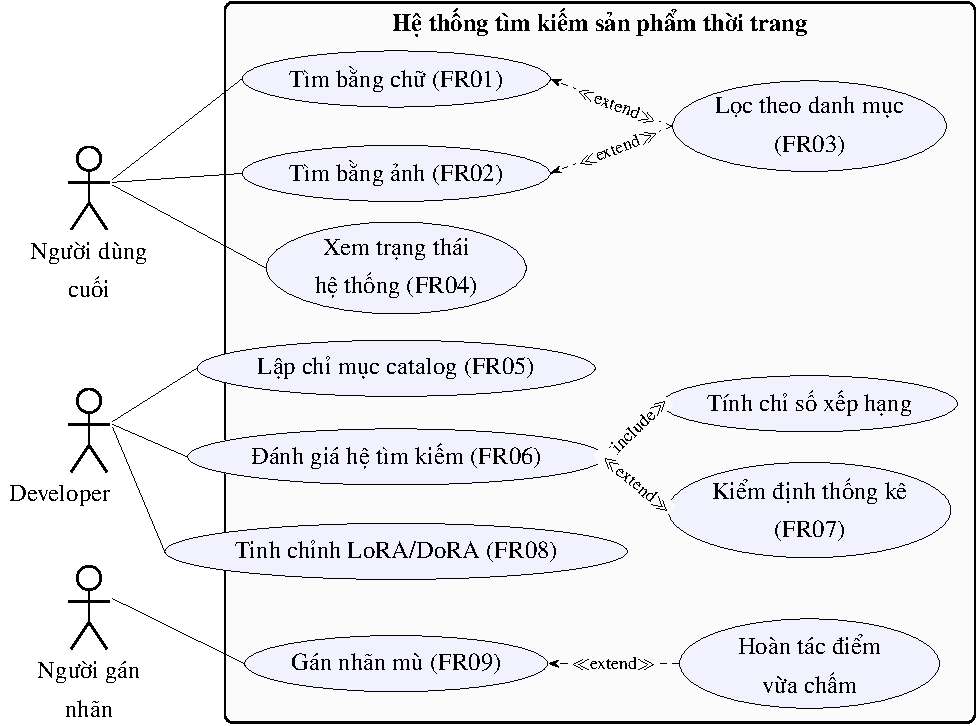
\includegraphics[width=0.9\textwidth]{graphics/fig_ch3_1.pdf}
\caption{Sơ đồ chức năng theo ba nhóm tác nhân}
\label{fig:c3_chucnang}
\end{figure}

\begin{table}[!htbp]
\centering
\caption{Kịch bản UC01, tìm sản phẩm bằng mô tả chữ}
\label{tab:c3_uc01}
\footnotesize
\renewcommand{\arraystretch}{1.05}
\begin{tabularx}{\textwidth}{@{}p{3.0cm} >{\raggedright\arraybackslash}X@{}}
\toprule
\textbf{Chức năng} & Tìm sản phẩm bằng mô tả chữ (FR01, FR03) \\
\midrule
\textbf{Tác nhân} & Người dùng cuối \\
\midrule
\textbf{Điều kiện ban đầu} & API web đang chạy với một bộ tìm kiếm đã cấu hình; catalog đã được lập chỉ mục \\
\midrule
\textbf{Luồng chính} & 1. Người dùng nhập mô tả, chẳng hạn ``áo len dệt kim xám'', rồi nhấn nút Tìm.\newline
2. Giao diện gửi mô tả cùng số kết quả mong muốn tới API web.\newline
3. API web kiểm tra khoá (nếu máy chủ bật khoá) và độ dài mô tả.\newline
4. Bộ tìm kiếm mã hoá câu và lấy từ kho các vector gần nhất.\newline
5. Giao diện hiển thị lưới thẻ kết quả theo hạng, mỗi thẻ có ảnh, tiêu đề, danh mục và độ tương đồng \\
\midrule
\textbf{Luồng rẽ nhánh} & 1a. Người dùng chọn một danh mục: yêu cầu mang thêm bộ lọc theo tên danh mục.\newline
1b. Người dùng đã chọn một ảnh trước đó: nút Tìm chạy kịch bản UC02 thay cho kịch bản này \\
\midrule
\textbf{Ngoại lệ} & Bước 1: ô mô tả trống và chưa chọn ảnh, giao diện nhắc nhập mô tả và không gửi yêu cầu.\newline
Bước 3: khoá API sai, API web trả 401.\newline
Bước 4: kho vector không phản hồi, API web trả 503.\newline
Bước 5: không có sản phẩm nào khớp bộ lọc, giao diện gợi ý đổi mô tả hoặc bỏ bộ lọc \\
\midrule
\textbf{Kết quả} & Người dùng nhận tối đa $K$ sản phẩm xếp theo độ gần với mô tả \\
\bottomrule
\end{tabularx}
\end{table}

\begin{table}[!htbp]
\centering
\caption{Kịch bản UC02, tìm sản phẩm bằng ảnh}
\label{tab:c3_uc02}
\footnotesize
\renewcommand{\arraystretch}{1.05}
\begin{tabularx}{\textwidth}{@{}p{3.0cm} >{\raggedright\arraybackslash}X@{}}
\toprule
\textbf{Chức năng} & Tìm sản phẩm bằng ảnh mẫu (FR02, FR03) \\
\midrule
\textbf{Tác nhân} & Người dùng cuối \\
\midrule
\textbf{Điều kiện ban đầu} & Như UC01, và bộ tìm kiếm của cấu hình là loại vector; BM25 không mã hoá được ảnh \\
\midrule
\textbf{Luồng chính} & 1. Người dùng kéo ảnh vào vùng thả hoặc chọn tệp jpg, jpeg, png hay webp, rồi nhấn nút Tìm.\newline
2. Giao diện gửi ảnh cùng số kết quả mong muốn tới API web.\newline
3. API web kiểm tra khoá, ảnh không rỗng và dung lượng không quá 8 MiB.\newline
4. Bộ tìm kiếm mã hoá ảnh bằng chính bộ mã hoá đã lập chỉ mục catalog và lấy từ kho các vector gần nhất.\newline
5. Giao diện hiển thị lưới thẻ kết quả như ở UC01 \\
\midrule
\textbf{Luồng rẽ nhánh} & 1a. Người dùng bấm nút bỏ ảnh: giao diện quay về tìm bằng chữ.\newline
2a. Người dùng đã chọn danh mục: yêu cầu mang thêm trường danh mục \\
\midrule
\textbf{Ngoại lệ} & Bước 1: ảnh lớn hơn 8 MiB, giao diện từ chối ngay và không gửi.\newline
Bước 3: ảnh rỗng, API web trả 422; ảnh quá lớn mà vẫn tới được máy chủ, API web trả 413.\newline
Bước 4: cấu hình dùng BM25, API web trả 501; kho vector không phản hồi, API web trả 503 \\
\midrule
\textbf{Kết quả} & Người dùng nhận tối đa $K$ sản phẩm có vector gần vector của ảnh mẫu \\
\bottomrule
\end{tabularx}
\end{table}

\section{Kiến trúc hệ thống}
\label{sec:kien-truc}

\subsection{Các tầng của hệ thống}

Hình~\ref{fig:c3_kientruc} mô tả hệ thống theo mô hình cổng và bộ chuyển đổi~\cite{cockburn2005hexagonal}, gồm bốn tầng. Cổng là giao diện trừu tượng do lõi định nghĩa; bộ chuyển đổi là phần cài đặt cụ thể của một cổng.

\begin{itemize}
\setlength{\itemsep}{1pt}
\item Tầng 1 là các điểm vào: giao diện web cùng API web, công cụ lập chỉ mục, công cụ đánh giá (kể cả thí nghiệm loại bỏ từng thành phần), công cụ huấn luyện và công cụ gán nhãn.
\item Tầng 2 là lõi, gồm các thực thể của mô hình miền, các cổng và bộ tìm kiếm vector. Lõi chỉ dùng thư viện chuẩn nên chạy được khi chưa cài thư viện học máy nào.
\item Tầng 3 gồm các bộ chuyển đổi cài đặt cổng của lõi: mô hình nhúng, kho vector, bộ tìm kiếm từ khoá BM25 và bộ chỉ số. Phần huấn luyện và các phép kiểm định thống kê cũng thuộc tầng này nhưng không cài đặt cổng nào. Huấn luyện chỉ dùng thực thể sản phẩm; kiểm định là hàm bổ sung của bộ chỉ số.
\item Tầng 4 là tài nguyên bên ngoài: trọng số mô hình, trọng số bổ sung của LoRA, Qdrant, tệp catalog, ảnh, truy vấn, nhãn và nhật ký thí nghiệm.
\end{itemize}

\begin{figure}[!htbp]
\centering
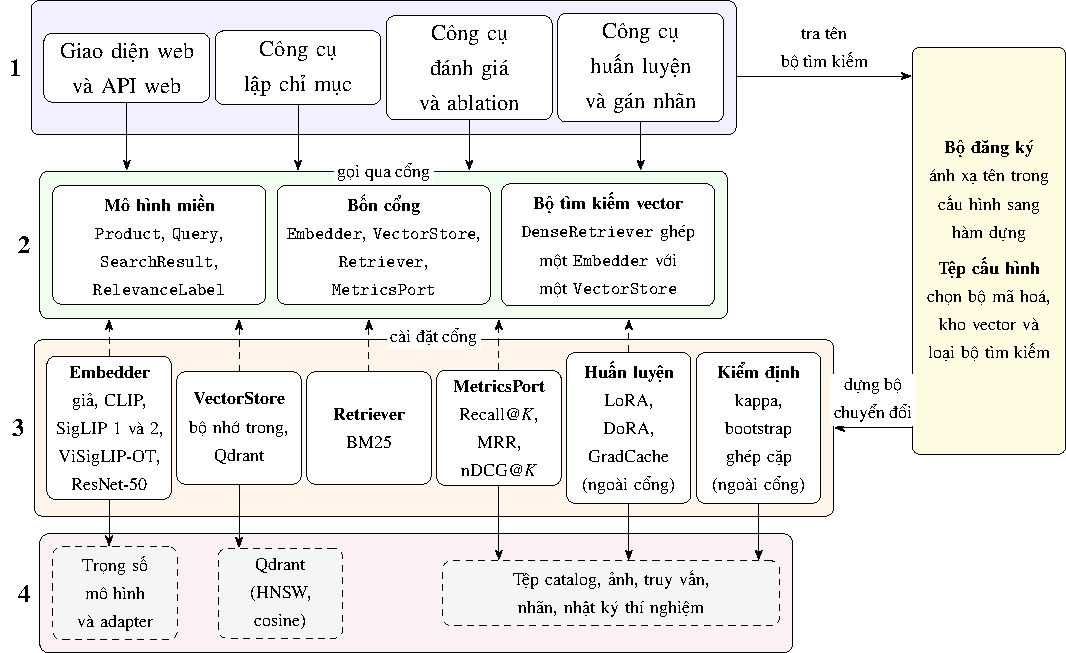
\includegraphics[width=\textwidth]{graphics/fig_ch3_2.pdf}
\caption{Kiến trúc bốn tầng theo mô hình cổng và bộ chuyển đổi}
\label{fig:c3_kientruc}
\end{figure}

Phụ thuộc đi một chiều: tầng 1 gọi lõi qua cổng, bộ chuyển đổi ở tầng 3 phụ thuộc vào cổng của lõi, còn lõi không biết bộ chuyển đổi nào tồn tại. Bộ đăng ký đọc tên trong tệp cấu hình và dựng bộ chuyển đổi tương ứng.

\subsection{Các lựa chọn thiết kế chính}

\begin{enumerate}
\setlength{\itemsep}{2pt}
\item \textbf{Bốn cổng ở lõi.} Lõi định nghĩa bốn cổng cho bộ mã hoá, kho vector, bộ tìm kiếm và bộ chỉ số. Mỗi mô hình, kho vector hay cách tìm kiếm là một bộ chuyển đổi cài đặt một cổng; nhờ vậy các hệ được so sánh trong chương đánh giá dùng chung một quy trình đánh giá (NFR03, NFR04).
\item \textbf{Cấu hình chọn bộ chuyển đổi.} Tệp cấu hình ghi tên bộ mã hoá, kho vector và loại bộ tìm kiếm; bộ đăng ký chỉ nạp các bộ chuyển đổi nặng khi được gọi tên. Cấu hình mặc định dùng bộ mã hoá mô phỏng 64 chiều và kho trong bộ nhớ, nên hệ thống khởi động được mà không cần GPU hay Qdrant (NFR02).
\item \textbf{Catalog được lập chỉ mục bằng ảnh.} Catalog chỉ có tên danh mục, không có mô tả màu hay chất liệu, nên vector của sản phẩm lấy từ ảnh. Công cụ lập chỉ mục gọi thẳng bộ mã hoá ảnh rồi ghi vector vào kho. Tài liệu của BM25 vì thế chỉ gồm tên danh mục tiếng Việt; Chương~\ref{chap:danh_gia} bàn hệ quả của điều này với việc so sánh các hệ.
\item \textbf{Hai kho vector cho hai mục đích.} Kho trong bộ nhớ tìm chính xác và được dùng để đánh giá, đo độ trễ; Qdrant tìm gần đúng bằng HNSW~\cite{malkov2020hnsw} và được dùng cho trình diễn. Các chỉ số đánh giá nhờ vậy không chịu ảnh hưởng của phép tìm gần đúng; mức chênh giữa hai kho nằm ở Mục~\ref{sec:han-che-danh-gia}.
\item \textbf{Truy vấn chữ và truy vấn ảnh xử lý riêng.} API web nhận truy vấn chữ hoặc truy vấn ảnh, không nhận cả hai cùng lúc, vì đồ án không hợp nhất vector chữ và vector ảnh. Truy vấn ảnh đi qua bộ mã hoá ảnh của chính mô hình SigLIP~2 đã tinh chỉnh đang phục vụ tìm bằng chữ, nên ảnh truy vấn và ảnh catalog nằm trong cùng không gian vector. Đồ án đánh giá truy vấn bằng chữ (Mục~\ref{sec:han-che-danh-gia}).
\end{enumerate}

\section{Các luồng xử lý chính}
\label{sec:luong-xu-ly}

\subsection{Lập chỉ mục catalog}

Luồng lập chỉ mục (Hình~\ref{fig:c3_hoatdong}) bắt đầu bằng việc đọc cấu hình và danh sách sản phẩm, rồi dựng bộ mã hoá và kho qua bộ đăng ký. Chế độ mã hoá bằng ảnh chỉ chạy với bộ tìm kiếm vector; nếu cấu hình dùng loại khác, công cụ dừng trước khi xoá hay ghi bất cứ dữ liệu nào. Tiếp theo, bộ sưu tập được tạo nếu chưa có, hoặc xoá rồi tạo lại khi người dùng yêu cầu. Với mỗi lô, công cụ mã hoá ảnh thành vector chuẩn hoá $L_2$ và ghi vào kho kèm thuộc tính sản phẩm. Chạy lại cùng catalog thì sản phẩm cũ bị ghi đè chứ không nhân đôi. Khi gặp ảnh không đọc được, công cụ dừng, báo mã sản phẩm và giữ nguyên các lô đã ghi.

\begin{figure}[!htbp]
\centering
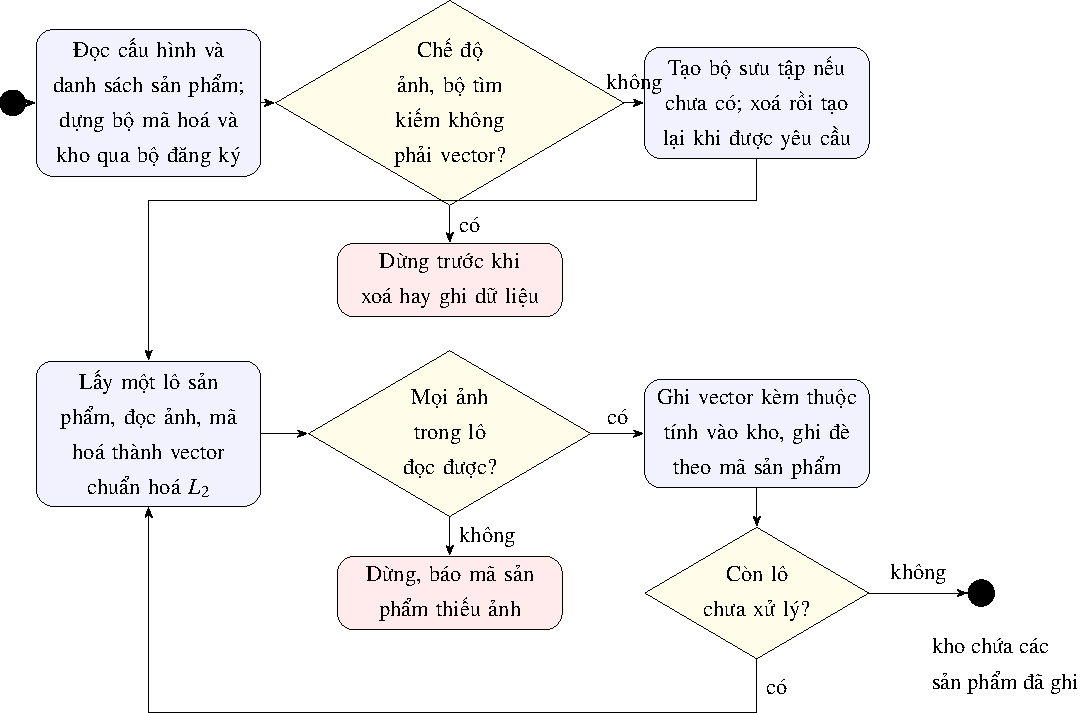
\includegraphics[width=0.85\textwidth]{graphics/fig_ch3_3.pdf}
\caption{Biểu đồ hoạt động của luồng lập chỉ mục catalog}
\label{fig:c3_hoatdong}
\end{figure}

\subsection{Tìm kiếm bằng chữ}

Hình~\ref{fig:c3_tuantu} là biểu đồ tuần tự của một truy vấn chữ. API web kiểm tra đầu vào rồi tạo một đối tượng truy vấn với mã ngẫu nhiên, số kết quả và bộ lọc. Bộ tìm kiếm vector chuẩn hoá câu về dạng NFC và chữ thường, rồi gọi bộ mã hoá để đổi câu thành vector chuẩn hoá $L_2$. Sau đó nó lấy từ kho $K$ sản phẩm gần nhất theo độ tương đồng cosine, kèm bộ lọc danh mục nếu có. Các trường hợp lỗi nằm ở Bảng~\ref{tab:c3_uc01}. Luồng tìm bằng ảnh chỉ khác ở bước mã hoá. Với BM25, bộ tìm kiếm tự chấm điểm theo từ, không qua bộ mã hoá và kho.

\begin{figure}[!htbp]
\centering
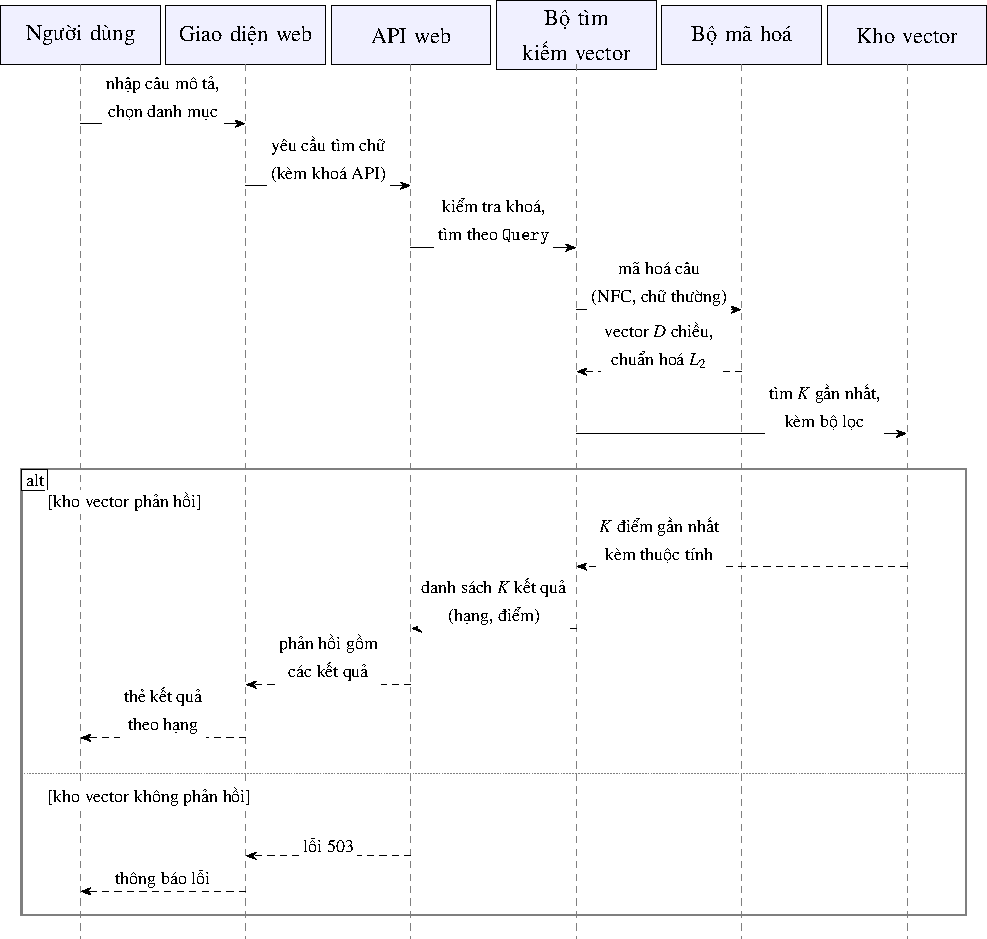
\includegraphics[width=0.88\textwidth]{graphics/fig_ch3_4.pdf}
\caption{Biểu đồ tuần tự của luồng tìm kiếm bằng chữ}
\label{fig:c3_tuantu}
\end{figure}

\section{Các thành phần chính}
\label{sec:thanh-phan}

Hình~\ref{fig:c3_lop} vẽ bốn cổng, bộ tìm kiếm vector của lõi (tô xanh) và các bộ chuyển đổi. Hệ thống có bốn bộ mã hoá dùng trong đánh giá: bộ mô phỏng 64 chiều, CLIP 512 chiều, SigLIP~2 768 chiều và ViSigLIP-OT 768 chiều; kèm hai kho vector, bộ tìm kiếm BM25 và bộ tính chỉ số xếp hạng.

Bộ mã hoá SigLIP~2 cũng nạp được SigLIP~1 khi đổi tên bản trọng số; danh sách mô hình cụ thể nằm ở Bảng~\ref{tab:c4_mahoa}. Bộ tìm kiếm vector thuộc lõi: nó ghép một bộ mã hoá với một kho vector để cài đặt cổng tìm kiếm, nên mọi cặp bộ mã hoá và kho đều dùng chung bộ này. BM25 cài đặt cùng cổng nhưng giữ chỉ mục riêng và không dùng kho.


\begin{figure}[!htbp]
\centering
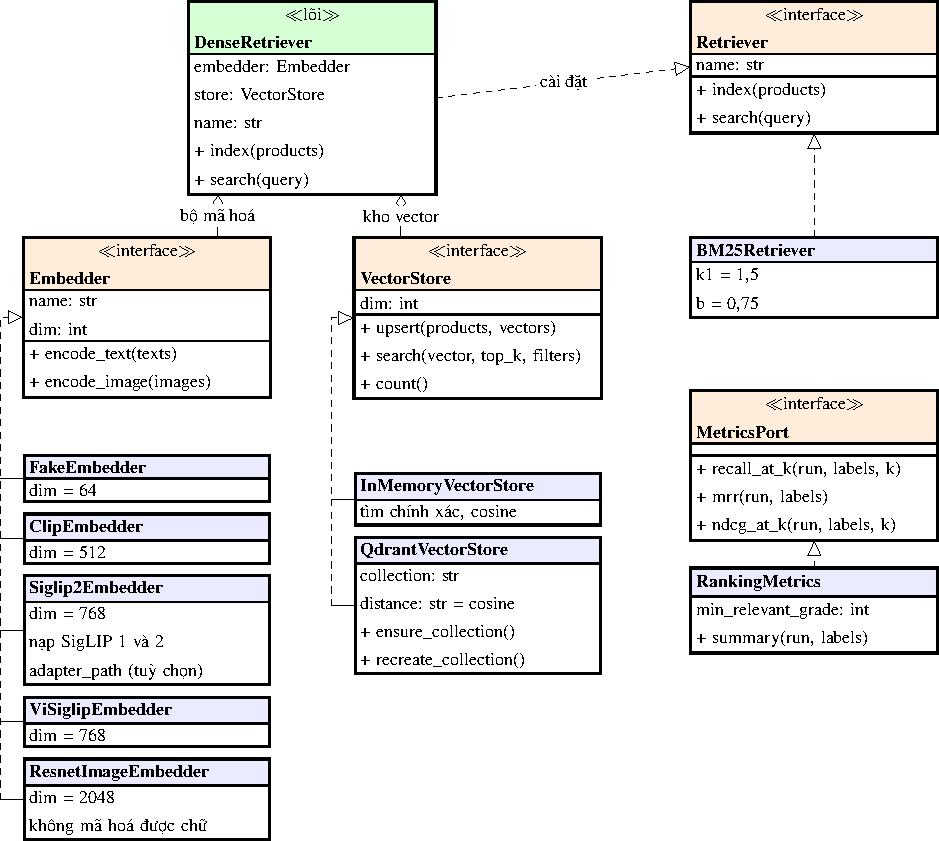
\includegraphics[width=0.86\textwidth]{graphics/fig_ch3_5.pdf}
\caption{Biểu đồ lớp của các cổng và bộ chuyển đổi}
\label{fig:c3_lop}
\end{figure}

\section{Cơ sở dữ liệu}
\label{sec:co-so-du-lieu}

\subsection{Các thực thể và quan hệ}

Hệ thống không dùng cơ sở dữ liệu quan hệ; dữ liệu nằm ở các tệp văn bản và ở kho vector (Hình~\ref{fig:c3_erd}). Một truy vấn của bộ đánh giá có nhiều kết quả và nhiều nhãn; một sản phẩm xuất hiện trong nhiều kết quả và nhiều nhãn; mỗi sản phẩm có một vector trong mỗi bộ sưu tập của kho vector. Khi đánh giá, hệ thống ghi 20 kết quả đầu của từng hệ kèm mã truy vấn và tên hệ. Các bản ghi này hợp thành tập cặp cần chấm, tức các cặp truy vấn--sản phẩm chờ gán nhãn.

\begin{figure}[!htbp]
\centering
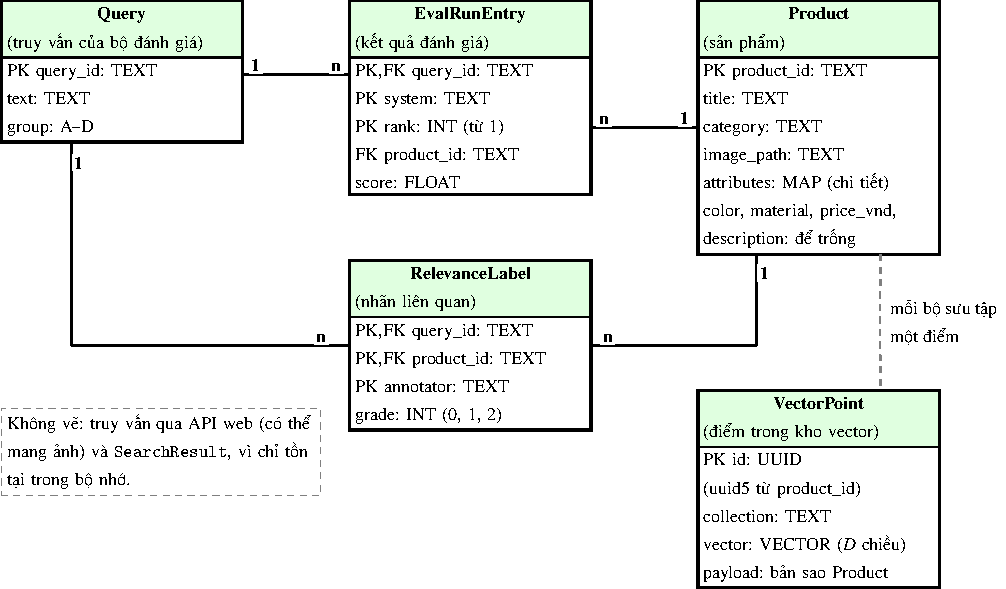
\includegraphics[width=0.88\textwidth]{graphics/fig_ch3_6.pdf}
\caption{Mô hình dữ liệu logic của hệ thống}
\label{fig:c3_erd}
\end{figure}

\subsection{Mô tả các bảng}

Bảng~\ref{tab:c3_thucthe} mô tả các thực thể. Về nơi lưu, catalog đã chuẩn bị, bộ 155 truy vấn và tập cặp cần chấm là các tệp JSON; nhãn của người chấm là các tệp JSONL, mỗi người một tệp, chỉ ghi nối thêm; nhật ký thí nghiệm là một tệp CSV 16 cột; vector sản phẩm nằm trong bộ sưu tập của kho.

Mỗi sản phẩm trong catalog chỉ có tên, danh mục, đường dẫn ảnh và chi tiết bộ phận trong trường thuộc tính. Màu, chất liệu, giá và mô tả để trống vì nguồn dữ liệu không có. Nhãn tự động do bộ lọc chấm 0 tạo ra (Mục~\ref{sec:du-lieu-cach-do}) luôn có điểm 0 và mang tên \texttt{auto-filter} ở cột người chấm. Bộ chỉ số coi cặp nằm trong $K$ kết quả đầu mà chưa có nhãn là không liên quan, đồng thời báo số cặp thiếu nhãn. Do đó Recall@10 là cận dưới của giá trị thật (Chương~\ref{chap:danh_gia}).

\begin{table}[!htbp]
\centering
\caption{Các thực thể của mô hình dữ liệu}
\label{tab:c3_thucthe}
\footnotesize
\renewcommand{\arraystretch}{1.05}
\begin{tabularx}{\textwidth}{@{}p{3.1cm} >{\raggedright\arraybackslash}X >{\raggedright\arraybackslash}X@{}}
\toprule
\textbf{Thực thể} & \textbf{Trường chính} & \textbf{Ràng buộc} \\
\midrule
\texttt{Product} & \texttt{product\_id}, \texttt{title}, \texttt{category}, \texttt{image\_path}, \texttt{attributes}, và bốn trường tuỳ chọn \texttt{color}, \texttt{material}, \texttt{price\_vnd}, \texttt{description} & Mã và tiêu đề không rỗng; giá không âm \\
\texttt{Query} & \texttt{query\_id}, \texttt{text}, \texttt{image\_bytes}, \texttt{image\_path}, \texttt{top\_k}, \texttt{filters}; ở bộ đánh giá có thêm \texttt{group} (nhóm A đến D) & Mã truy vấn không rỗng; có chữ hoặc ảnh; \texttt{top\_k} $\geq 1$ \\
\texttt{SearchResult} & \texttt{product}, \texttt{score}, \texttt{rank} & Hạng đánh số từ 1; chỉ có trong bộ nhớ, không lưu \\
\texttt{EvalRunEntry} & \texttt{query\_id}, \texttt{system}, \texttt{rank}, \texttt{product\_id}, \texttt{score} & Khoá là (\texttt{query\_id}, \texttt{system}, \texttt{rank}); mỗi hệ giữ 20 kết quả đầu \\
\texttt{RelevanceLabel} & \texttt{query\_id}, \texttt{product\_id}, \texttt{grade}, \texttt{annotator} (tên người chấm, hoặc \texttt{auto-filter} với nhãn tự động) & Điểm thuộc $\{0, 1, 2\}$ \\
\texttt{VectorPoint} & mã bản ghi trong kho, vector $D$ chiều ($D$ do bộ mã hoá quyết định), bản sao thuộc tính sản phẩm & Ở Qdrant, mã là \texttt{uuid5} của \texttt{product\_id}; kho trong bộ nhớ khoá thẳng theo \texttt{product\_id}; mỗi bản trọng số có một bộ sưu tập \\
\bottomrule
\end{tabularx}
\end{table}

\section{Giao diện người dùng}
\label{sec:giao-dien}

Giao diện web là một màn hình duy nhất, không chuyển trang (Hình~\ref{fig:c3_dieuhuong}): thanh trên hiện trạng thái hệ thống, hai phần tìm bằng chữ và bằng ảnh cùng hiển thị kết quả trên một lưới.

\begin{figure}[!htbp]
\centering
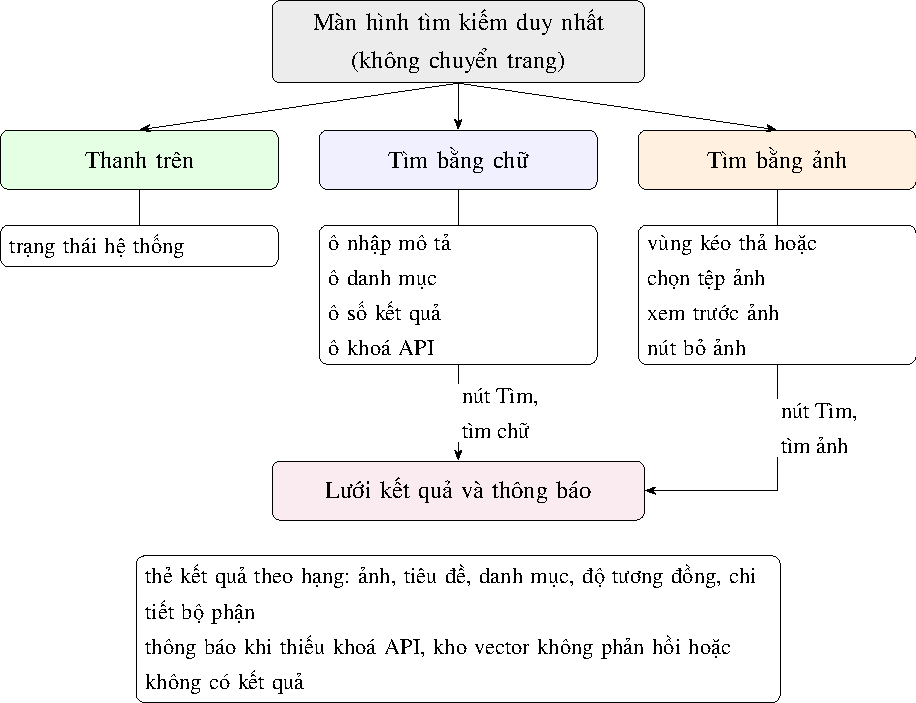
\includegraphics[width=0.66\textwidth]{graphics/fig_ch3_7.pdf}
\caption{Sơ đồ điều hướng của giao diện web}
\label{fig:c3_dieuhuong}
\end{figure}

Giao diện dùng một nút Tìm cho cả hai cách: khi đã chọn ảnh thì tìm theo ảnh, nếu không thì tìm theo chữ, nên người dùng không phải chuyển chế độ. Lỗi hiện bằng lời tiếng Việt theo từng nguyên nhân (Bảng~\ref{tab:c3_uc01} và \ref{tab:c3_uc02}).
